
\newcommand{\irow}[1]{% inline row vector
\big[ \  #1 \ \big]%
}

\chapter{Punkteverarbeitung}

3D-Objekte werden oft durch Scheitelpunkte und Dreiecke dargestellt, welche deren dreidimensionale Form widerspiegelt.
Dabei gilt, je detaillierter ein Objekt ist, desto mehr Scheitelpunkte werden benötigt. Bei einem Objekt wie dem
Menschen mit weitgehend vordefinierter Form kann die Darstellung jedoch auf einige wenige Größen wie Höhe,
Dicke, Brustumfang, Bauchgröße und Pose reduziert werden. Diese Darstellung ist oft kleiner und aussagekräftiger.
\cite{Ha2018} Die Idee ist die Entwicklung einer Funktionalität, welche die Rückgabewerte der
Messfunktion als Eingangsparameter für die Erstellung eines Modells mit STAR nutzbar macht.

\section{STAR}

Eine dieser Darstellungen ist der Sparse Trained Articulated Human Body Regressor (STAR). 
STAR ist ein statistisches Modell, das den menschlichen Körper mit zwei Parametern, dem Shape-Parameter $\boldsymbol{\beta}$
für die Form und dem Pose-Parameter $\boldsymbol{\Theta}$ für die Pose, beschreibt.

\subsection{Shape}

Einer der beiden Parameter für die Generierung des Modells eines menschlichen Körpers mit STAR ist der sogenannte Shape-Parameter.
Dieser umfasst 10 bis 300 Skalare \linebreak ${\boldsymbol{\beta}= \irow{\beta _0 \ ,\ \ldots \ , \ \beta_{|\beta|}}}$, welche die
Form des menschlichen Körpers widerspiegeln. Jedes Skalar erwirkt bei der Modellgenerierung eine
Veränderung eines bestimmten Merkmals. Das Skalar $\beta _0$ ist dabei beispielsweise ausschlaggebend
für die Größe des Modells, $\beta _1$ wirkt auf das Verhältnis von Körpergröße und Gewicht, ähnlich wie
der Body Mass Index. Der Wert für $\beta _2$ bestimmt die Höhe des Torsos und Schulterbreite, jener für
$\beta _3$ die Brustbreite sowie Nackenhöhe.
\begin{figure}[H]
  \centering 
   \subfigure[negativ]{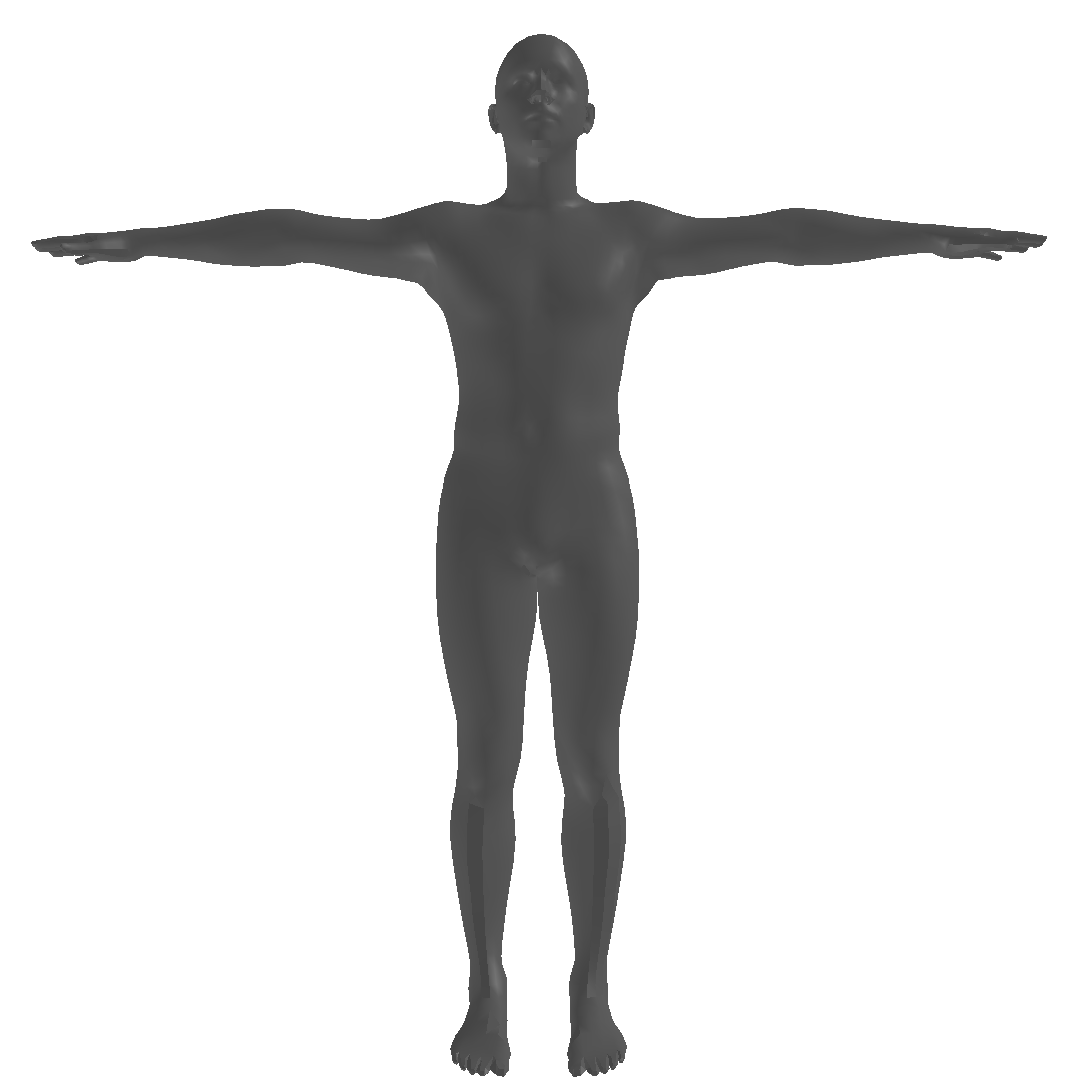
\includegraphics[width=0.4\textwidth]{shape_slim}}\qquad 
   \subfigure[positiv]{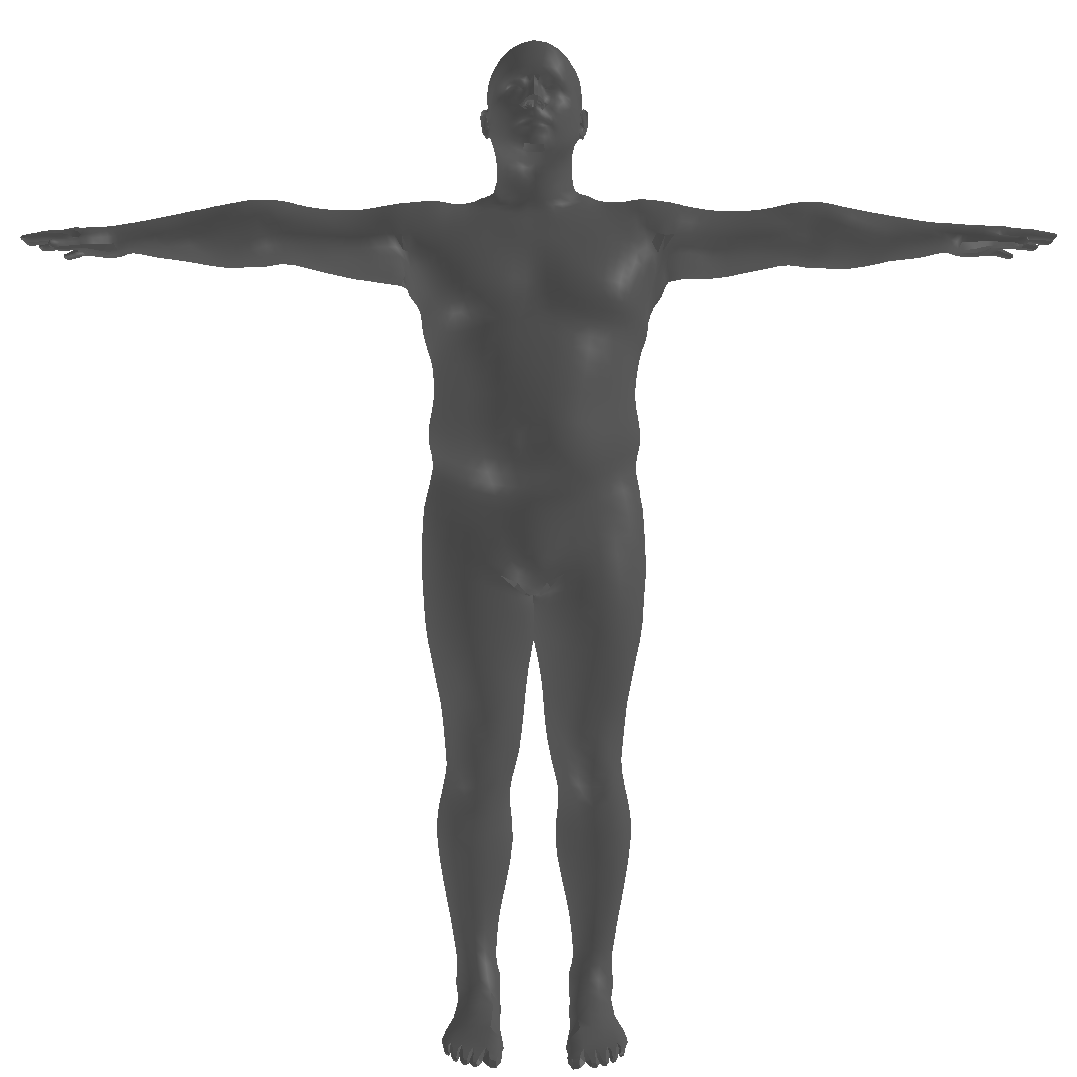
\includegraphics[width=0.4\textwidth]{shape_big}}\qquad 
   \subfigure[default (=0)]{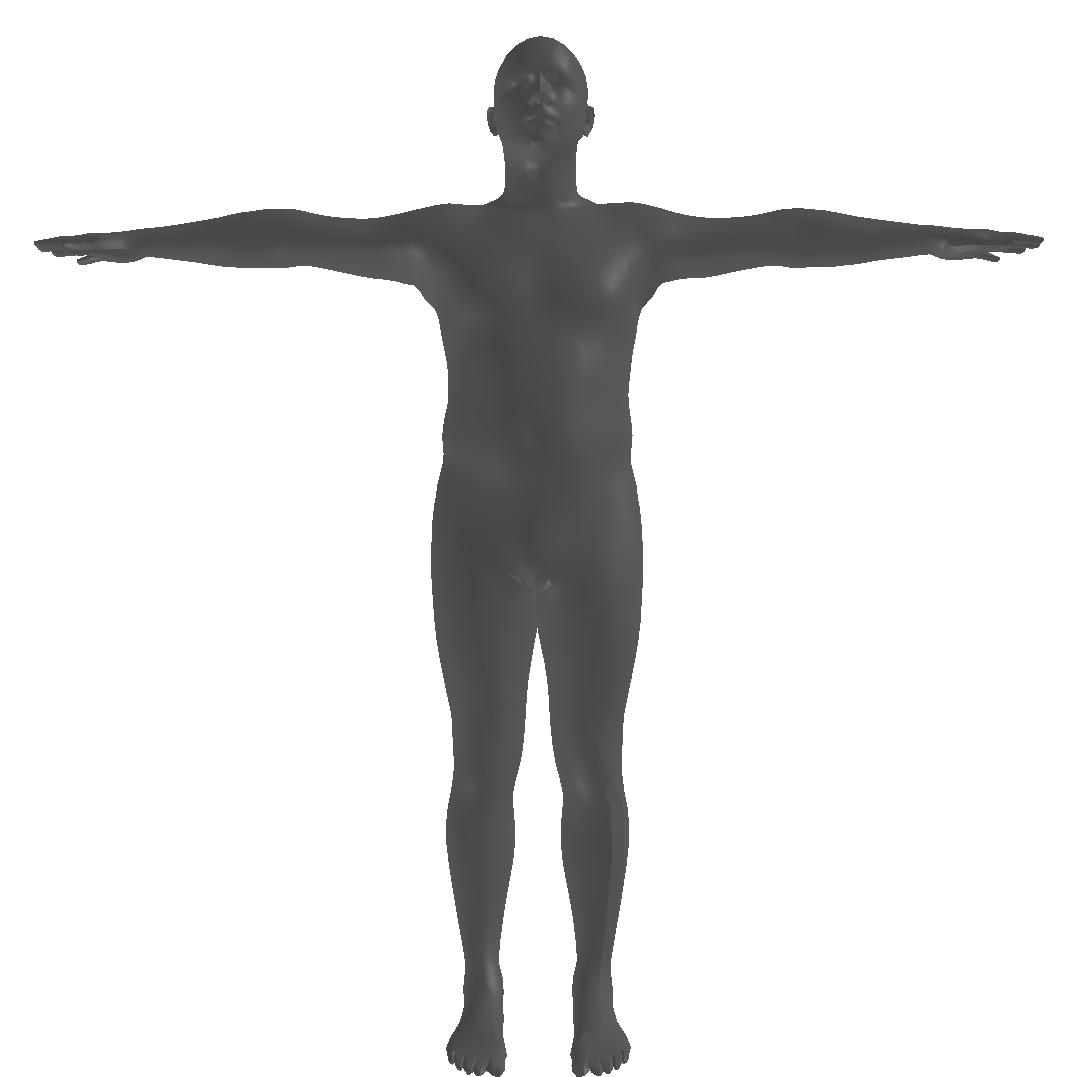
\includegraphics[width=0.4\textwidth]{shape_normal}}
  \caption{Gerenderte Modelle mit verschiedenen Shape-Parametern} 
  \label{fig:betas}
\end{figure}

Ein negativer Wert für einen Skalar reduziert dabei das
entsprechende Merkmal, ein positiver Wert verstärkt dieses (vgl. Abb. \ref{fig:betas}). Je höher dabei die Anzahl an Skalaren,
desto genauer lässt sich das Modell an einen bestimmten Körperbau anpassen, im Gegenzug
erhöht sich aber der Rechenaufwand.

\subsection{Pose}

Der zweite Eingabeparameter für STAR ist der Pose-Parameter, welcher die zu generierende Pose
mit 24 Vektoren ${\boldsymbol{\Theta}=\irow{\vec{\Theta} _0 \ ,\ \ldots \ , \ \vec{\Theta} _{23}}}$, die
je 3 Skalare ${ \vec{\Theta} _n=\irow{x_n \ ,\ y_n \ ,\ z_n}}$ umfassen, beschreibt. Die Vektoren
werden als Rotation in Axis-Angle-Darstellung von Gelenken des menschlichen Körpers relativ
zum Vorgängergelenk interpretiert, welche zusammengesetzt einen sogenannten Kinematischen
Baum mit den wichtigsten Gelenkpunkten ergeben (vgl. Abb. \ref{fig:axisangle}, (b)). Die Axis-Angle-Darstellung
beschreibt die Drehung eines dreidimensionalen Objekts um den Winkel $\Theta$ um eine Rotationsachse
mit dem Einheitsvektor $\vec{e}$. Diese beiden Variablen können mit $\Theta * \vec{e}$ als Vektor mit drei Parametern und dem Betrag $\boldsymbol{\Theta}$
zusammengefasst werden. (vgl. Abb. \ref{fig:axisangle}, (a)).

\begin{figure}[H]
  \centering 
   \subfigure[]{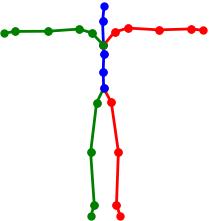
\includegraphics[width=0.45\textwidth]{joints}}\qquad
   \subfigure[]{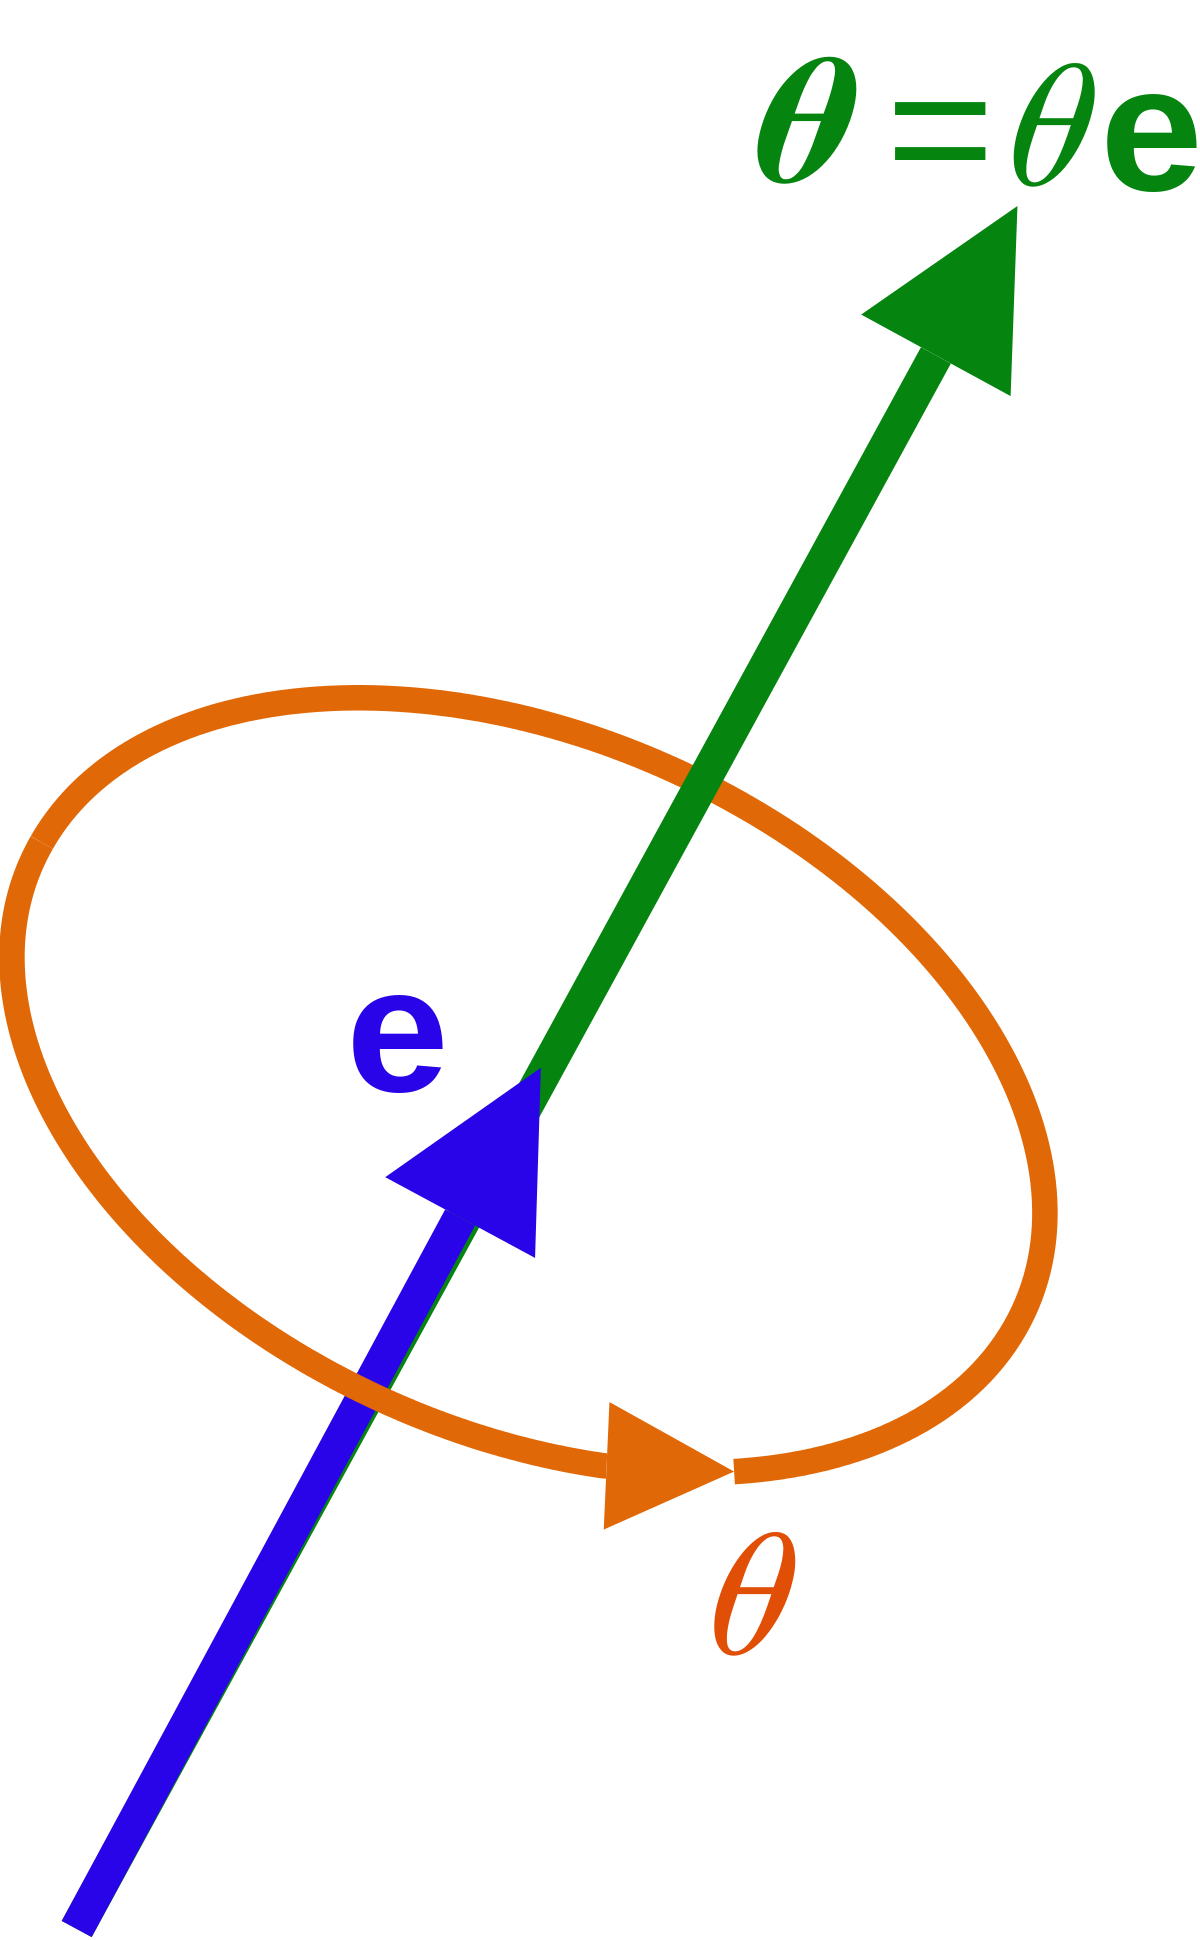
\includegraphics[width=0.3\textwidth]{Angle_axis_vector}}
  \caption{Gelenke des STAR-Modells (a) und Axis-Angle-Darstellung einer Rotation \cite{wiki:Axis–angle_representation} (b)} 
  \label{fig:axisangle}
\end{figure}

\newpage
Dabei gilt, je kleiner der Wert eines Skalars gegenüber den anderen beiden Skalaren, desto geringer
ist die Drehung entlang der entsprechenden X-Achse, Y-Achse oder Z-Achse. Eine Drehung um $\frac{\pi}{2}$ um die
X-Achse und $\frac{\pi}{2}$ um die Y-Achse entspräche $\irow{0.89*\frac{\pi}{2} \ ,\ 0.45* \frac{\pi}{2} \ ,\ 0}$ in 
Axis-Angle-Darstellung. Durch verschiedene Gewichtungen der 24 Vektoren kann so jede erdenkliche Pose
dargestellt werden (vgl. Abb. \ref{fig:poses}, (b)). Sind die Elemente eines Vektors $\vec{\Theta _n} = \irow{0 \ , \ 0 \ ,\ 0}$, befindet sich das Gelenk in Ruheposition.
Abbildung \ref{fig:poses} (a) zeigt das Modell, bei dem sich alle Gelenke in Ruhepose befinden.

\begin{figure}[H]
  \centering 
   \subfigure[Ruhepose]{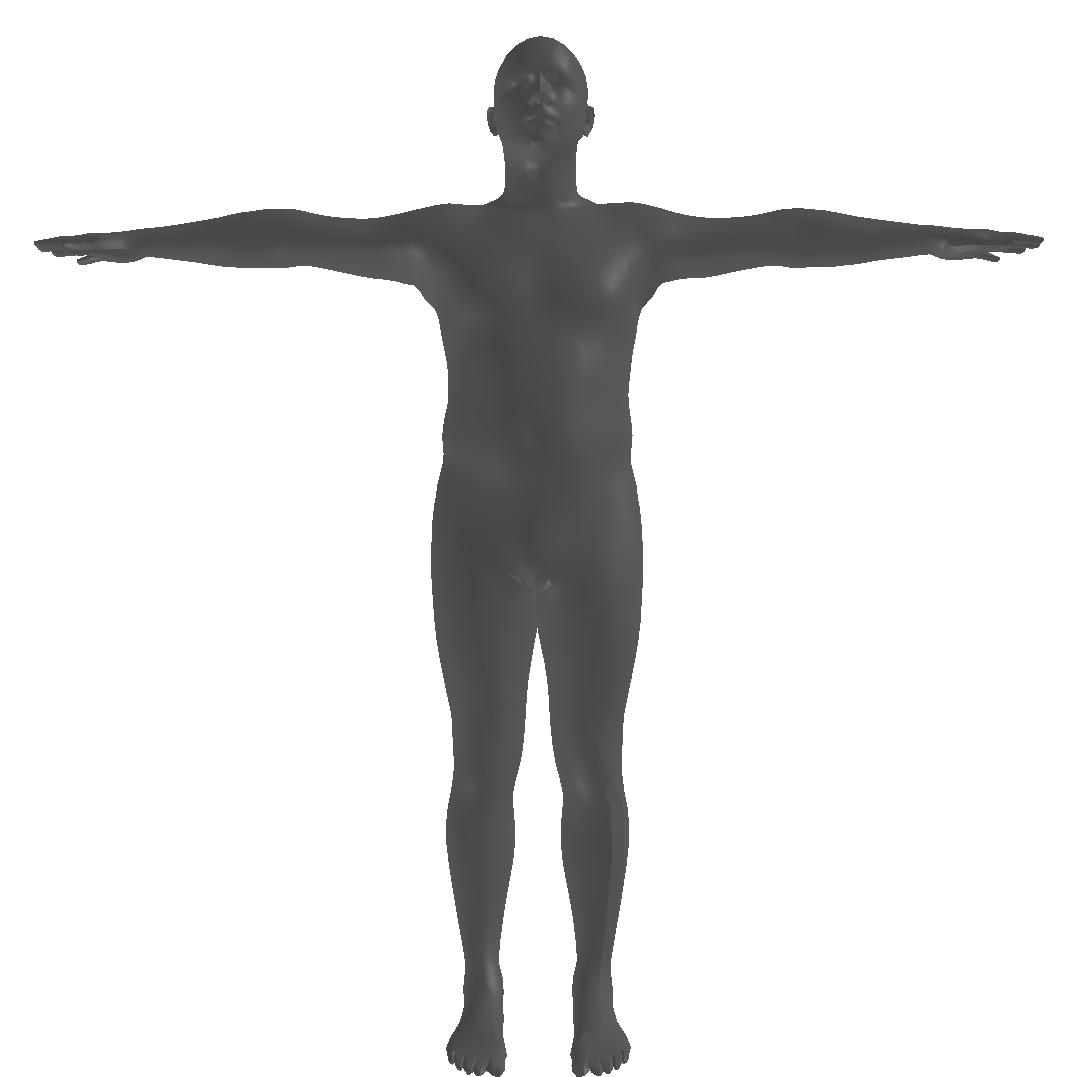
\includegraphics[width=0.4\textwidth]{pose0}}\qquad 
   \subfigure[Zufällige Pose]{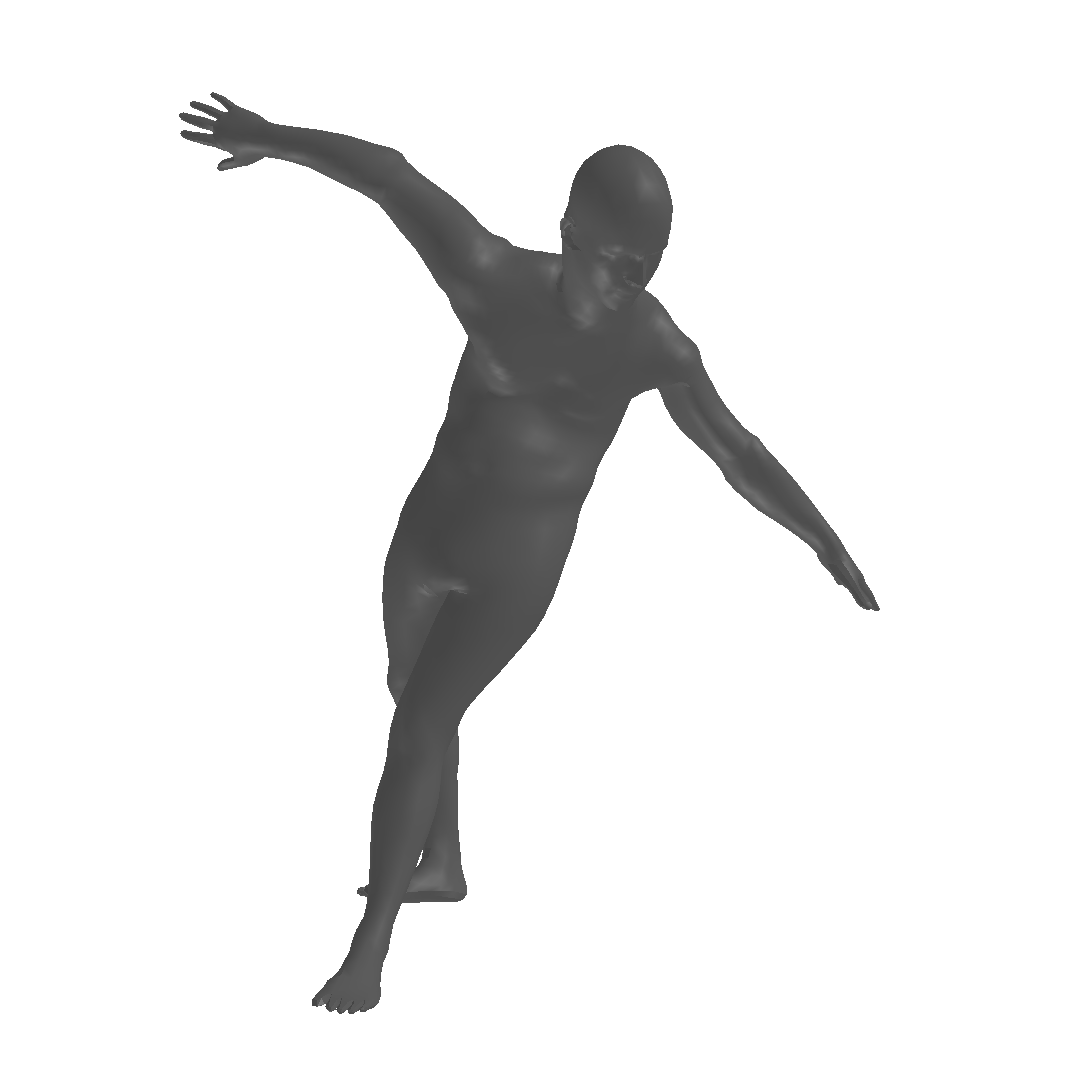
\includegraphics[width=0.4\textwidth]{pose1}}
  \caption{Gerenderte Modelle mit verschiedenen Pose-Parametern} 
  \label{fig:poses}
\end{figure}

\subsection{Funktionsweise}

Die Pipeline der Synthese des menschlichen Körpers mit Star erfolgt in drei Schritten. In einem ersten Schritt wird ein
Template-Modell $\overline{T}$ in Ruhepose und ohne Form-Korrekturen erstellt und Scheitelpunktversätze zum Modell T mit der Funktion
$B_s(\beta;S)$ berechnet. Der Parameter $S$ beschreibt dabei vordefinierte grundlegende Komponenten, welche den Bereich der
menschlichen Formvariabilität erfassen. Addiert ergeben Modell $\overline{T}$ und Scheitelpunktversätze
$\vec{V}_{shaped}$, ein Modell in Ruhepose,
das die mit den Shape-Koeffizienten definierten physikalischen Attribute und die Identität widerspiegelt.

\begin{equation}\label{eq:Star_Vshaped}
  \vec{V}_{shaped}=\overline{T}+B_s(\beta;S)
\end{equation}

Der menschliche Körper verformt sich in unterschiedlichen Posen anders, was für ein realistisches Ergebnis in Betracht
gezogen werden muss. Diese Verformung ist zudem abhängig von der Form des Körpers. Der zweite Schritt dient dementsprechend der
Berechnung der durch die Pose $\Theta$ verursachten Verformungen in Korrelation mit den Shape-Koeffizienten $\beta$ durch die Funktion
$B_p(\vec{q},\beta _1) $. Der Parameter $\vec{q}$ stellt dabei den kinematischen Baum als Quaternion mit je vier
Parametern pro Skelettpunkt dar. $\beta _1$, also der
zweite Koeffizient des Shape-Parameters, ist repräsentativ für die allgemeine Form des Körpers und stimmt in vielen
Punkten mit dem Body Mass Index (BMI) überein. Da $\beta _1$ den mit Abstand größten Einfluss auf die Verformungen durch
spezielle Posen hat, können die restlichen Shape-Koeffizienten vernachlässigt werden. Das Endresultat $\vec{V}_{posed}$, gegeben
durch

\begin{equation}\label{eq:Star_Vposed}
  \vec{V}_{posed}=\overline{T}+B_s(\beta;S)+B_p(\vec{q},\beta _1)
\end{equation}

stellt nun ein Modell in Ruhepose dar, das sowohl Verformungen durch den Shape-Parameter als auch durch den
Pose-Parameter umfasst. Da das Modell $\vec{V}_{posed}$ posenspezifische Verformungen umfasst, aber trotzdem in Ruhepose dargestellt
wird, kann ein leicht unförmiger Eindruck entstehen. 

Im dritten und letzten Schritt, dem sogenannten Skinning, wird das Mesh mit einer standard skinning Funktion $\mathcal{W}$  um die Joints von $\vec{V}_{shaped}$ transformiert sowie durch ein erlerntes Set aus blend weight parametern geglättet. Das Modell ist schlussendlich gegeben durch

\begin{equation}\label{eq:Star_Model}
  M(\vec{\beta},\vec{\Theta})=W(T_p(\vec{\beta},\vec{\Theta}), J(\vec{\beta},\vec{\Theta}, \mathcal{W}))
\end{equation}

Die Funktion $J$ regressiert dabei die Joints zwischen den Skelettpunkten aus $\vec{V}_{shaped}$. Das so synthetisierte Modell des
menschlichen Körpers ist realistisch und weicht bei richtiger Messung und Parametrierung von Shape und Pose um nur wenige
Millimeter ab. Ziel des folgenden Kapitels ist die Entwicklung einer Funktionalität, welche die Rückgabewerte der
Messfunktion als Eingangsparameter für die Erstellung eines Modells mit STAR nutzbar macht.

\section{Verarbeitung}

Um mittels Star ein realistisches Modell des menschlichen Körpers zu generieren, müssen die Rückgabewerte der
Measure-Funktion zu Shape-Parameter $v{\beta}$ und Pose-Parameter $\boldsymbol{\Theta}$ konvertiert werden. Im Folgenden wird die Idee der Konvertierung, die Umsetzung sowie aufgetretene
Probleme dargestellt.

\subsection{Idee}

In allen großen Messpunkten des Zozosuits befindet sich eine einzigartige Punkteanordnung, wodurch jedem gescannten
Messpunkt eine ID und somit eine entsprechende Position auf dem Zozosuit zugewiesen werden kann. Diese ID wird von der Measure-Funktion, neben den genauen Koordinaten und einer geschätzten Entfernung des
Punktes, erfasst. Dadurch lässt sich eine dreidimensionale Punktewolke erzeugen und die genauen Koordinaten eines
Messpunktes auf dem Zozosuit mit der ID ermitteln.

Die Pose kann so durch Zuweisung von passenden Punkten des Zozosuits zu den Gelenkpunkten des
Pose-Parameters rekonstruiert werden. Hierfür ist es erforderlich, die Rotation in
Axis-Angle-Darstellung zu berechnen, welche den Vektor zwischen zwei Gelenkpunkten des kinematischen Baums der Ruhepose zu dem 
Vektor zwischen den zwei entsprechenden Punkten auf dem Zozosuit rotiert.

Die Ermittlung des Shape-Parameters erweist sich als komplexer. Die bis zu 300 verschiedenen Skalare, welche auch in
gegenseitiger Wechselwirkung stehen, zu erschließen, ist mit den Daten, die die Messfunktion des Zozosuit liefert,
unmöglich. Allerdings könnte man nur einige wenige der Skalare betrachten, welche einen großen Einfluss auf die
allgemeine Form haben, wie die Skalare $\beta _0$ und $\beta _1$, welche die Größe sowie den Body Mass Index des Modells beschreiben. Diese können 
durch Messung von Entfernungen verschiedener bestimmter Punkte grob bestimmt werden. Dies soll aber im Rahmen
der Arbeit dieser Arbeit nicht näher betrachtet werden.

\subsection{Umsetzung}
Für die Ermittlung der Pose aus den Daten der Zozosuit-Messfunktion erfolgt in 
einem ersten Schritt die Zuweisung der IDs von Messpukten zu den Gelenkpunkten des Pose-Parameters.
 Dies wird einmalig durch einen Vergleich von Gelenkpunkten des Kinematischen Baums und 
Messpunkten auf dem Zozosuit ermittelt.

\begin{figure}[H]
  \centering 
   \subfigure[Erfasste Punkte]{\includegraphics[width=0.3\textwidth]{point_positions}}\qquad 
   \subfigure[Nummerierte Joints des STAR-Modells \cite{STAR:2020}]{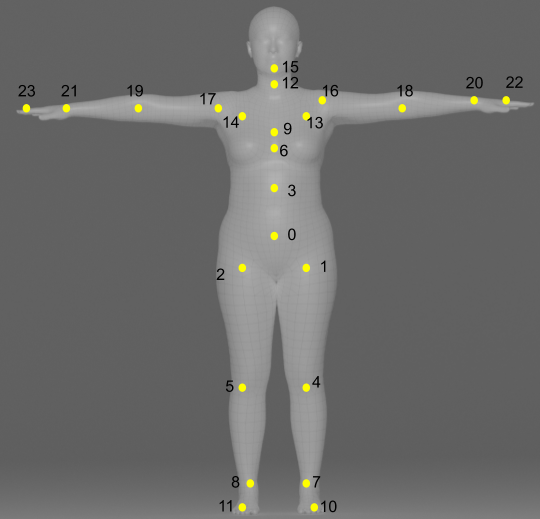
\includegraphics[width=0.6\textwidth]{star_kinematic_tree}}
  \caption{Vergleich von Joints des Star-Modells und Punkten des Zozosuits mit IDs in Gelb} 
  \label{fig:pointpos}
\end{figure}

Die Koordinaten der Messpunkte, deren ID mit einem Gelenkpunkt verknüpft ist, werden aus dem Rückgabewert
\texttt{raw\_data} als dreidimensionale Punktewolke ausgelesen. Da der Pose-Parameter Rotationen von Gelenk zu 
übergeordnetem Gelenk gemäß des kinematischen Baums benötigt, ist eine Konvertierung der Punktewolke zu Rotation in 
Axis-Angle-Darstellung erforderlich. Die Rotation eines Gelenks wird dabei relativ zur Rotation des Gelenks in Ruhepose berechnet.
In anderen Worten muss die Rotation des Vektors \texttt{v\_src} von übergeordnetem Gelenkpunkt zu Gelenkpunkt
der Ruhepose zu Vektor \texttt{v\_dst} von übergeordnetem Gelenkpunkt zu Gelenkpunkt der Messpose berechnet werden. Hierfür dient die
Funktion \texttt{axis\_angle(v\_src,v\_dst)}, welche die Rotation von \texttt{v\_src} zu \texttt{v\_dst} in Axis-Angle-Darstellung zurückgibt.

In der Funktion \texttt{axis\_angle(\dots)} werden in einem ersten Schritt werden beide Vektoren genormt, da lediglich
die Richtung der Vektoren bei der Berechnung der Rotationsmatrix eine Rolle spielen. Die Rotationsachse
ist definiert durch das Kreuzprodukt von Ursprungsvektor und Zielvektor, der Winkel der Drehung durch den
Arkustangens des Skalarprodukts der beiden Vektoren. Demnach lässt sich die Drehung eines Vektors 
$\vec{v}_{src}$ zu einem Vektor $\vec{v}_{dst}$ in Axis-Angle-Darstellung mit

\begin{equation}\label{eq:axis_angle}
  \boldsymbol{\Theta} = \Theta * \vec{e} = \arctan(\vec{v}_{src} \cdot \vec{v}_{dst}) * \lVert \vec{v}_{src} \times \vec{v}_{dst} \rVert
\end{equation}

berechnen. Nachdem dies für alle Gelenke berechnet wird, lässt sich mit Hilfe von Star ein Modell generieren, welches
die Pose der Person auf dem Bild widerspiegelt. Allerdings treten dabei einige Probleme auf, die das Ergebnis
stark verzerren können, welche im Folgenden vorgestellt werden.

\subsection{Probleme}
\label{subsec:probleme}
Bei der Synthese der Pose aus den Messpunkten des Zozosuit treten eine Reihe von Problemen auf.

\subsubsection*{Fehlende Messpunkte an Gelenken}
Ein Problem ist, dass nicht für jedes Gelenk ein Messpunkt auf dem Zozosuit existiert. Einige
Gelenke müssen deshalb komplett ausgelassen werden, wie beispielsweise jene an Kopf, Füßen und Händen, da kein Messpunkt in der
Nähe existiert. Diese sind für die gesamte Pose aber nicht ausschlaggebend. Deshalb wird für diese die Ruhepose des Gelenkes
$\boldsymbol{\Theta}=\irow{0 \ , \ 0 \ ,\ 0}$ verwendet. Bei anderen Gelenken, vor allem in der Schulterregion liegen die Messpunkte
lediglich in der Nähe des Gelenks (vgl. Abb. \ref{fig:schulter}).

\begin{figure}[H]
  \centering 
   \subfigure[Erfasste Punkte in der Schulterregion]{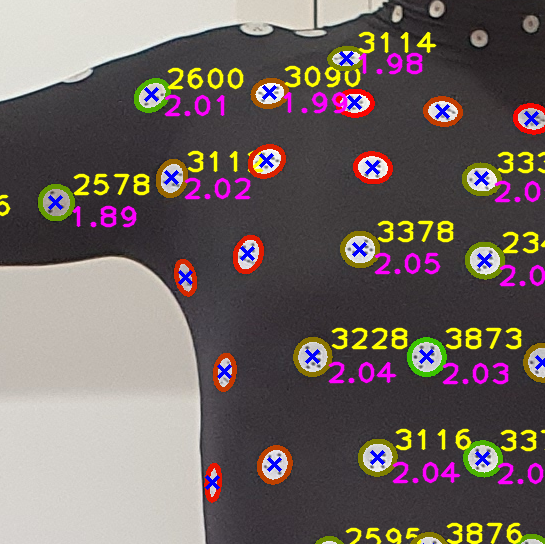
\includegraphics[width=0.475\textwidth]{point_positions_schulter}}\qquad 
   \subfigure[Gelenke in der Schulterregion \cite{STAR:2020}]{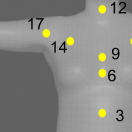
\includegraphics[width=0.475\textwidth]{star_kinematic_tree_schulter}}
  \caption{Vergleich von Joints des Star-Modells und Punkten des Zozosuits mit IDs in gelb} 
  \label{fig:schulter}
\end{figure}

Dadurch wird die Pose verzerrt, Beispiele hierfür sind leicht falsch abstehende Arme oder gespreizte Beine. Zwar können 
einige Gelenke durch Zusammenspiel von mehreren Messpunkten berechnet werden, allerdings 
wird der Effekt durch das nachfolgend beschriebene Problem verstärkt.

\subsubsection*{Lückenhafte Punkterkennung}
Bei der Erkennung der Messpunkte mit der Zozosuit-Messfunktion werden häufig Punkte gar nicht oder ohne
ID erkannt. Die dadurch entstehende lückenhafte dreidimensionale Punktewolke der Messpose hat zur Folge, dass
nicht alle Pose-Parameter berechenbar sind. Jeder fehlende Messpunkt, mit Ausnahme der Start- und Endpunkte, 
verursacht zwei fehlende Pose-Parameter, die zur Ruhepose des Gelenks gesetzt werden müssen. Dadurch kommt es teils
zu einer Pose des Modells, die einigen essenziellen Aspekten gar nicht mit der Pose des Menschen auf dem Bild übereinstimmt.
So kann eine fehlerhafte Erkennung des Messpunktes für ein Schultergelenk dazu führen, dass der Arm des Modells 
waagerecht (Ruhepose) steht, und nicht wie auf dem Bild dargestellt.
Wird versucht, Gelenke mit mehreren Messpunkten zu beschreiben, steigt dabei 
die Wahrscheinlichkeit für fehlende berechenbare Pose-Parameter, sodass dies keine Lösung zum ersten Problem darstellt.


\subsubsection*{Verzerrung durch Drehung des Zozosuits}
Ein weiteres Problem ist, dass sich der Zozosuit nach dem Anziehen oft leicht verdreht ist. Dadurch liegen die
vordefinierten Messpunkte nicht genau auf den entsprechenden Gelenken, oder können teils gar nicht erkannt werden,
da diese nun im toten Winkel der Kamera liegen. Dies verursacht häufig gespreizte beziehungsweise verdrehte Beine oder einen 
verdrehten Oberkörper sowie eine lückenhafte Erkennung der Punkte in der Armregion, was eine Darstellung der Arme
in Ruhepose zur Folge hat. Zwar kann diese Fehlerquelle durch korrekten Sitz des Zozosuits teilweise verhindert werden,
allerdings verbleibt meistens eine Restdrehung.


\subsubsection*{Fehlerhafte Erkennung der ID}
Die wohl gravierendste Fehlerquelle besteht in der falschen Erkennung der ID eines Messpunktes. Teilweise weist die
Zozosuit-Messfunktion einem Messpunkt eine falsche ID zu. Ist der Messpunkt jener falsch erkannten ID einem 
Gelenk zugewiesen, kann dies gravierende Folgen für das generierte Modell haben. Je nach Lage des Messpunktes
mit der falschen ID kann das Gelenkt stark verdreht werden, was eine groteske Darstellung des Gelenks im Modell
zur Folge hat. Das Modell zeigt dadurch teilweise einen in Teilen deformierten menschlichen Körper,
beispielsweise mit einem grotesk verdrehten und abstehendem Bein, was bei den vorgenannten Problemen nicht auftreten kann.
Bei jenen wird zwar die Pose oft nicht richtig widergespiegelt, allerdings verkörpert die gezeigte Pose im Modell eine
reale, nachstellbare Pose.
